\begin{frame}
  \frametitle{Solving partial differential equations}
  It's a tough job!

  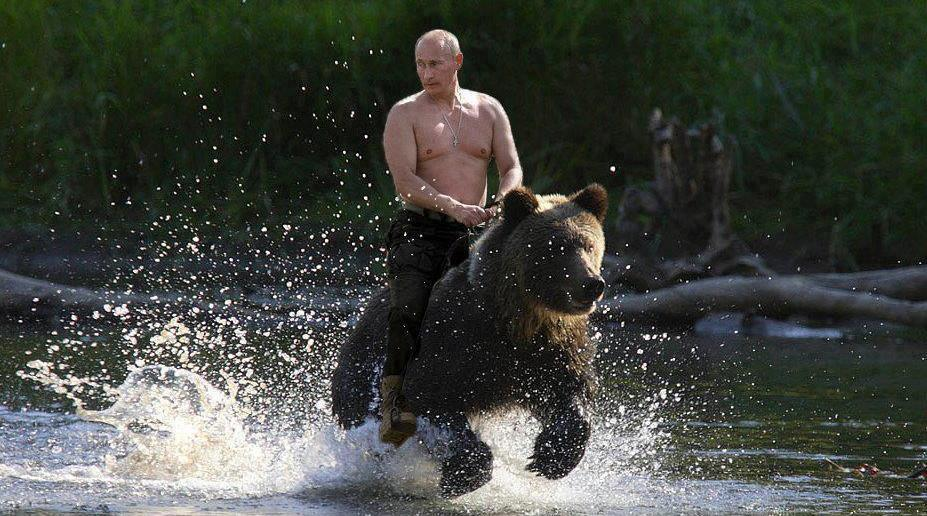
\includegraphics[width=\columnwidth]{putin}
\end{frame}

\begin{frame}{Options}
\begin{enumerate}
\item Crank-Nicholson
\item Iterative mesh techniques

  Update grid untill PDE is fullfilled in all points. 
\end{enumerate}
\end{frame}


\begin{frame}
  \frametitle{Crank-Nicholson}
  Applies for diffusion problems:
  \[  \pdiff{u}{t} = F \Big(u, x, t, \pdiff{u}{x}, \ppdiff{u}{x} \Big). \]
  Utilize the equality of forward- and backwards Euler method.
  \begin{center}
    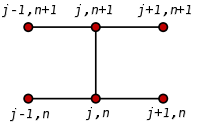
\includegraphics[width=0.4\columnwidth]{Crank}
  \end{center}
\end{frame}

\begin{frame}{Finite difference}

Use discrete version of differential operators

\begin{align*}
  f'(x) &= \frac{f(x+\half h) - f(x - \half h)}{h}\\[5mm]
  f''(x) &= \frac{f(x+h) - 2f(x) + f(x-h)}{h^{2}}.
\end{align*}

Introduce unitless quantities and assume cylindrical beam
\[   i \pdiff{\tilde E}{\tilde z} + \ppdiff{\tilde E}{\tilde r}
+ \frac{1}{\tilde r} \pdiff{\tilde E}{\tilde r}
+ |\tilde E|^2 \tilde E
= 0,\]
  
\end{frame}

\begin{frame}
  \frametitle{End result}
  A "almost" five diagonal matrix system.
  $n$ is z direction, $i$ is radial direction
  
  \begin{align*}
    (\alpha + 2\beta^{2} - |E_{i}^{n+1}|^{2})E_{i}^{n+1} - \beta^{2}(E_{i+2}^{n+1} + E_{i-2}^{n+1}) -
    \frac{\beta}{r_{i}} (E_{i+1}^{n+1} - E_{i-1}^{n+1}) \\
    = (\alpha - 2\beta^{2} + |E_{i}^{n}|^{2})E_{i}^{n} + \beta^{2}(E_{i+2}^{n} + E_{i-2}^{n}) +
    \frac{\beta}{r_{i}} (E_{i+1}^{n} - E_{i-1}^{n}),
  \end{align*}


  By approximating $|E_{i}^{n+1}|^{2} \approx |E_{i}^{n}|^{2}$ this is a matrix problem.

  This must be solved for every step!


  \vfill
  $\alpha = -2i/\!{\Delta z}$ and $\beta = 1/{2 \Delta r}$.

\end{frame}

\begin{frame}
  \frametitle{Well....}
  We could not fix numerical problems in $r = 0$. \bigskip

  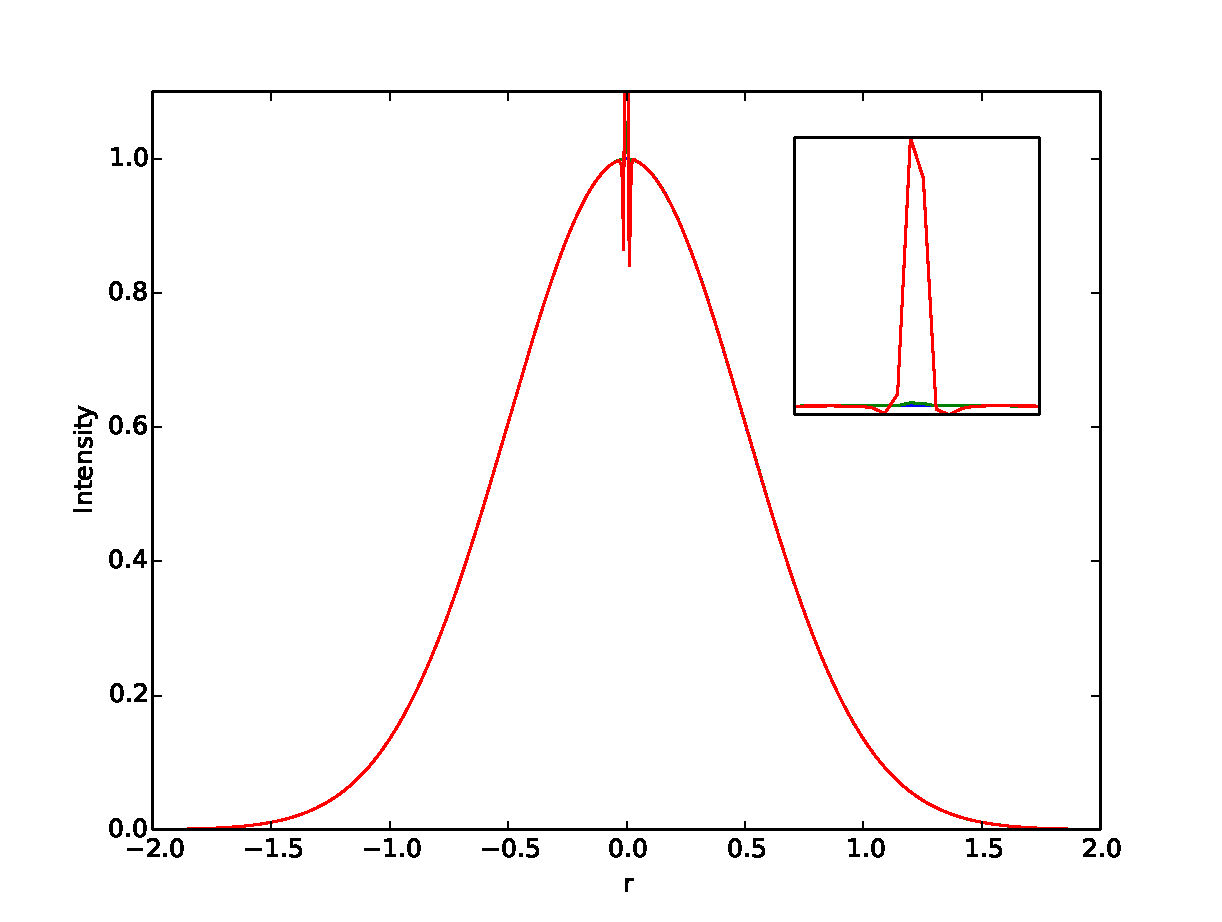
\includegraphics[width=0.45\columnwidth]{kerr_double} \hfill 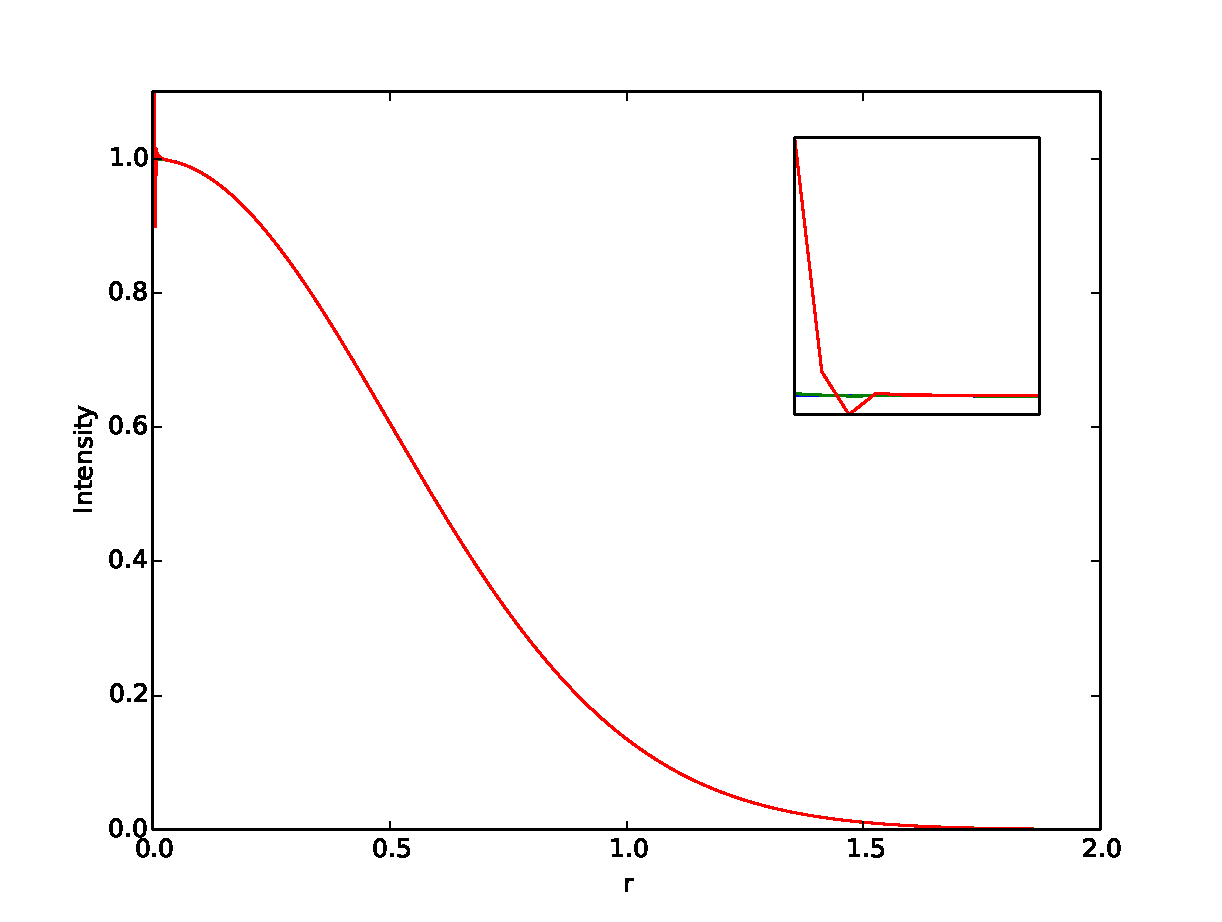
\includegraphics[width=0.45\columnwidth]{kerr_single}

  The iterative mesh technique requires us to solve a $N_{z} \times N_{r}$ set of nonlinear
  equations.

  We didn't have time to do this....
\end{frame}
%%% Local Variables: 
%%% mode: latex
%%% TeX-master: "nonlinearslides"
%%% End: 
